\chapter{Analysis Overview}
\label{ch:analysisOverview}


This chapter provides an overview of the analysis described in Chapter \ref{ch:analysis} and published in 2017\cite{stop0L13tev}.  As described in Chapter \ref{ch:motivations}, the search for the stop is well-motivated since the stop should be lighter than other squarks.  As it has the highest impact on naturalness, and could be the lightest squark, the stop is an important particle for which to perform a search.  Additionally, the lightest supersymmetric particle, e.g. the neutralino, is a viable dark matter candidate and is produced in conjunction with the stop in $R$-parity conserving SUSY models.  This dissertation describes a search for {\bf direct} stop pair production (in contrast to top squarks produced through gluino cascade decays).  Figure \ref{fig:stopCS} shows the direct production cross section of the stop quark as a function of its mass with several SM processes shown for comparison.  \\%\color{red}{Some more motivation here?}\color{black}{}

%   the large Yukawa couplings tend to drive down the masses of the third generation squarks in the renormalization group equations faster than the first two generations\cite{susyprimer}.  Additionally, the large Yukawa couplings make the masses of the third generation squarks have the largest impact on the mass of the Higgs; if naturalness is to be maintained then their masses should be small relative to the cutoff scale.  \\

%While it is the lightest squark it still has a small production cross section and thus searches are challenging.  



\begin{figure}[h]
	\centering
	\includegraphics[width=.5\textwidth,trim={0 0 0 0},clip]{stopCS_1.pdf}
	\caption[Cross section for direct stop pair production and selected backgrounds.]{\label{fig:stopCS}{Cross section for direct stop pair production as a function of stop mass at a center-of-mass energy of 13 TeV.  Several SM cross sections, $t\bar{t}$, $Z+$jets\cite{ttZcs}, and $tt+Z$\cite{ttZcs}, are shown as well for reference.  Note that for heavier stop quarks SM processes have cross sections that are orders of magnitude larger.}}
\end{figure}

 % where the mass of the top squark (\stop) is larger than the mass of the top quark ($t$): $m_{\stop} > m_t$. 
%The search is performed in the channel
%$pp \rightarrow \stop\, {\stop}^{\ast}$, where two decay modes are
%possible for the stop decay:
%
%\begin{itemize}
%\item $\stop \rightarrow t + \ninoone$, or
%\item  $\stop \rightarrow b + \chinopm \rightarrow b + W^{(\ast)} + \ninoone$.
%\end{itemize}
%

Three different decay scenarios are considered in this search: (a) both top squarks decay via $\stop\rightarrow t^{(*)} \ninoone$, (b) at least one of the top squarks decays via $\stop\rightarrow b \chinoonepm \rightarrow b W^{(*)}\ninoone$, with various hypotheses for $\mLSP$ and $m_{\chinoonepm}$, and (c) where $m_{\ninotwo}$ is small enough for at least one top squark to decay via $\stop\to t \ninotwo \to h/Z \ninoone$, where $h$ is the SM-like Higgs boson with a mass of 125 GeV, as illustrated in Figure~\ref{fig:feynDiagModels}(a)$-$(c), respectively. In addition to direct pair production, top squarks can be produced indirectly through gluino decays, as shown in Figure~\ref{fig:feynDiagModels}(d).  In all cases, the all-hadronic decay of the top quark (or of the W in the $b + W^{(\ast)}
+ \ninoone$ mode) is considered. Orthogonal searches also exist that
focus on the lepton+jets\cite{stop1L13tev} and dilepton\cite{stop2L13tev} decay modes of the top quark. \\


\begin{figure}[htb]
\begin{center}
\subfloat[$\stop\ra t^{(*)}\ninoone$]{\includegraphics[width=0.3\textwidth]{figures/intro/stst-bqqbqqN1N1-tt}}\hspace{0.05\textwidth}
\subfloat[$\stop\ra b\chinoonepm\ra b \Wboson^{(*)}\ninoone$]{\includegraphics[width=0.3\textwidth]{figures/intro/stst-bbWWN1N1}}\hspace{0.05\textwidth}
\subfloat[$\stop\ra t\ninotwo\to h/Z\ninoone$]{\includegraphics[width=0.3\textwidth]{figures/intro/stst-tbhWN1N1}}\hspace{0.05\textwidth}
\subfloat[$\gluino \ra t\stop\ra t\ninoone +$soft]{\includegraphics[width=0.3\textwidth]{figures/intro/gogo-tsofttsoftN1N1-stst}}\hspace{0.05\textwidth}
\end{center}
\caption[Top quark decay topologies.]{The decay topologies of the signal models considered with experimental signatures of four or more jets plus missing transverse momentum. Decay products that have transverse momenta below detector thresholds are designated by the term ``soft".}
\label{fig:feynDiagModels}
\end{figure}

%\begin{figure}[tbp]
%	\centering
%	\subfloat[Simple]{\includegraphics[width=1in]{placeholder}}\quad
%	\subfloat[Simple]{\includegraphics[width=1in]{placeholder}}\\	
%	\caption{Parentheses, newline separator.}
%\end{figure}

The all-hadronic top decay mode nominally
has six jets in the final state, but events with at least four reconstructed jets are considered. However, this channel has the feature that there are no
neutrinos in the final state, so the only intrinsic \met\ is from the
$\nino$s except possibly from semi-leptonic $b$ decays.  Therefore the experimental
signature is multiple jets and high \met.  \\
% Top categories

A common feature of all analyses studying a specific phenomenon is defining a region of phase space designed to have a significant excess of signal events compared to background events.  This is done by applying selections to sets of kinematic observables and is called a signal region (SR).  Several signal regions have been developed to optimize sensitivity to different stop-neutralino mass combinations, as illustrated in Figure \ref{fig:signalregions}, and different final states, as illustrated in Figure \ref{fig:feynDiagModels}. \\

\begin{figure}
\centering
	 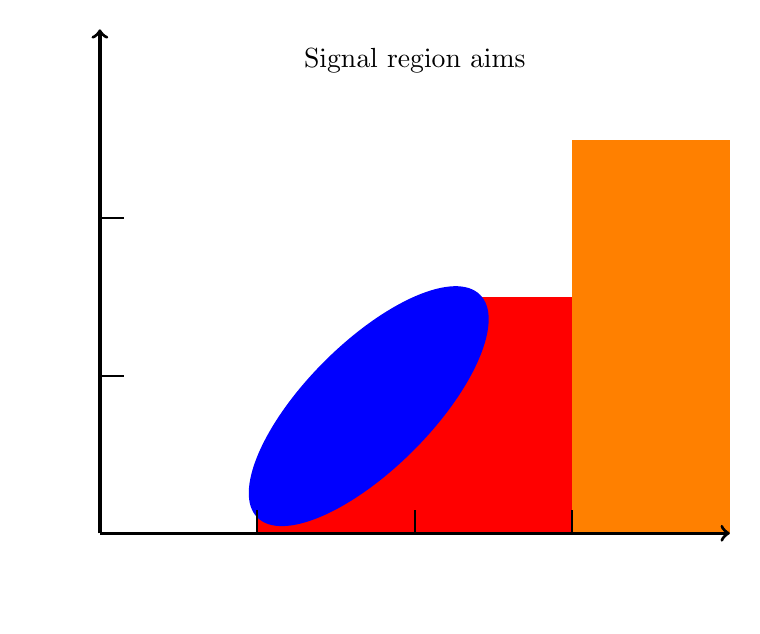
\begin{tikzpicture}[scale = 2]
          \draw[->,thick, line width=1.2] (0, 0) -- (0,3.2);
          \node[black] at (-0.4,2.7) {\mLSP};
          \draw[line width=0.8] (0, 1) -- (0.15,1);
          \draw[line width=0.8] (0, 2) -- (0.15,2);
          %\node[black] at (-0.2,1) {\tiny 100};
          %\node[black] at (-0.2,2) {\tiny 200};
          \fill [orange] (3,0) rectangle (4,2.5);
          \fill [red] (2,0) rectangle (3,1.5);
          \fill [red] (1,0) rectangle (2,0.3);
          \fill [red] (1.5,0) rectangle (2,0.7);

          \fill [blue,rotate around={-135:(1,0.1)}] (1,0.1) arc(0:360:1 and 0.4);

          \draw[line width=0.8] (1, 0) -- (1,0.15);
          \draw[line width=0.8] (2, 0) -- (2,0.15);
          \draw[line width=0.8] (3, 0) -- (3,0.15);
          %\node[black] at (1,-0.1) {\tiny 200};
          %\node[black] at (2,-0.1) {\tiny 400};
          %\node[black] at (3,-0.1) {\tiny 600};
          \node[black] at (3.7,-0.4) {\mstop};
          \draw[->,thick, line width=1.2] (0, 0) -- (4,0);
          \node[black] at (2,3) {Signal region aims};	
        \end{tikzpicture}
\caption[Illustration of signal regions.]{Multiple signal regions have been developed to increase sensitivity in different stop and neutralino mass combinations: SRC in blue, SRB in red, and SRA in orange.} \label{fig:signalregions}
\end{figure}


More details on the SRs are presented in Section \ref{sec:srDefs}.  Signal regions A (SRA) and B (SRB) are optimized for high stop masses in the decay channel shown in Figure \ref{fig:feynDiagModels}(a).  SRA is optimized to be sensitive to decays of heavy stops into a top quark and a light \LSP. Events are divided into three categories based on the reconstructed top candidate mass (nominally 175 GeV), which was not done in the Run 1 analysis\cite{stop0LRun1}. The Run 1 analysis was performed on 20.1 \ifb\ at a center-of-mass energy of 8 TeV.  The TT category includes events with two well-reconstructed top candidates, the TW category contains events with a well-reconstructed leading \pt\ top candidate and a well-reconstructed subleading $W$ candidate (from the subleading $R=1.2$ reclustered mass), and the T0 category represents events with only a leading top candidate. This is shown in Figure \ref{fig:categories}, where the horizontal axis is the mass of the leading $R=1.2$ reclustered mass and the vertical axis is that of the second-leading $R=1.2$ reclustered mass. Optimizing the significance\footnote{Significance is defined as $\frac{S}{\sqrt{B}}$ where $S$ is the number of signal events and $B$ is the number of background events} in the categories showed an improvement in discovery significance compared to the combined optimization. \\


\begin{figure}[t]
  \begin{center}
    \includegraphics[width=0.7\textwidth]{figures/SRA/CategoryDefs}
    \caption[Top quark mass categories.]{Illustration of signal-region categories (TT, TW, and T0) based on the $R=1.2$ reclustered top-candidate masses for simulated direct top-squark pair production with $(m_{\stop},m_{\ninoone})=(1000,1) \GeV$ after the loose preselection requirement described in the text. The black lines represent the requirements on the reclustered jet masses.}
    \label{fig:categories}
  \end{center}
\end{figure}

In SRC the signature of stop decays when $\Delta m(\stop,\LSP)\sim m_{t}$ is significantly softer with low \met\ for the decay channel shown in Figure \ref{fig:feynDiagModels}(a). This decay topology is very similar to non-resonant \ttbar\ production making signal and background separation challenging. However, several kinematic properties can be exploited to separate stop decays from \ttbar\ when an ISR jet is present in the final state. These variables are described in Section \ref{sec:SRC}. \\

The selections for SRD are optimized for the decay of both pair-produced top squarks into a $b$ quark and a \chinoonepm\ as shown in Figure \ref{fig:feynDiagModels}(b). SRE is designed for a model for which the tops are highly boosted. Such signatures can either come from direct stop pair production with a very high stop mass, or in the gluino-mediated compressed-stop scenario with large \mgluino - \mstop\ as shown in Figure \ref{fig:feynDiagModels}(d). \\

%The analysis is also sensitive to gluino mediated stop production in the case where $\Delta(\mgluino, \mstop)$ is large but $\Delta(\mstop,\mLSP)$ is small. This results in a decay signature that is similar to direct stop production with highly boosted tops and high \met. \\

Background processes that contaminate SRs must also be estimated.  Control regions (CRs) are designed for each dominant background to be pure in that background and have as little signal contamination as possible.  Appendix \ref{sec:signalContamination} shows the signal contamination in each of the CRs and VRs.  These are compared to data and therefore must be orthogonal to the SRs, but still as close as possible kinematically in order to reduce uncertainties when extrapolating.  The CRs are defined for the major backgrounds in each SR to normalize the simulation to data and ensure the shapes of the simulated backgrounds match those of the data.  However, enough data is required in order to minimize the uncertainties in the normalization factors. \\

The dominant background sources are:

\begin{itemize}
\item $Z\rightarrow \nu \nbar$ plus additional $b$-jets, typically produced in a Drell-Yan process.  
\item Semileptonic $\ttbar$ events, which contain $\Wboson \to e/\mu/\tau \nu$ decays where the lepton is either lost or mis-identified as a jet (and have high \met\ due to the escaping neutrino).
\item $W\rightarrow \ell \nbar$ plus additional $b$-jets, 
\item $\ttbar+\Zboson$, where both tops decay hadronically and $\Zboson\rightarrow \nu \nbar$, and
\item $Wt$-channel single top decays, where one $W$ decays hadronically and one leptonically.
\end{itemize}

Figure \ref{fig:atlasbsmsummaryfiducialxsect} summarizes theory predictions and ATLAS measurements for various SM production cross-sections and shows both total and fiducial cross sections\footnote{A fiducial cross section is a cross section for the subset of a process which is visible in the detector.}.  \\




\begin{figure}[tbh!]
	\centering
	\includegraphics[width=0.9\linewidth]{figures/ATLAS_b_SMSummary_FiducialXsect}
	\caption[SM fiducial production cross sections.]{Summary of several SM total and fiducial production cross section measurements compared to the corresponding theoretical expectations\cite{atlassmsummaryplots}.}
	\label{fig:atlasbsmsummaryfiducialxsect}
\end{figure}

It can be seen in Figure \ref{fig:bkgSRB}, which shows the backgrounds in SRB, that $Z\rightarrow \nu \nbar$ and $\ttbar$ are major contributors to the background processes. \\


\begin{figure}[H] 
\begin{center}
 \includegraphics[width=0.2\textwidth]{figures/barCharts/bkgBarsSRB1.pdf} %\hspace{0.05\textwidth}
 \includegraphics[width=0.2\textwidth]{figures/barCharts/bkgBarsSRB2.pdf} %\hspace{0.05\textwidth}
 \includegraphics[width=0.2\textwidth]{figures/barCharts/bkgBarsSRB3.pdf} %\hspace{0.05\textwidth}
    \caption[Backgrounds in SRB.]{Breakdown of the backgrounds in SRB-TT, -TW, and -T0 from left to right.}
    \label{fig:bkgSRB}
\end{center}
\end{figure}

% CRs are designed to be orthogonal to all SRs while as close to the SR kinematically as possible to reduce uncertainties from the extrapolation.  To reduce uncertainties in normalization factors a lot of data is required.  

The strategy for the CRs are:

\begin{itemize}
	\item 1-lepton: Requires exactly one well-identified lepton in order to be orthogonal to the SRs and treat it as a jet.  This CR is used for leptonically-decaying $W$ bosons, as in the $t\bar{t}$, $W+$jets, and single top backgrounds.  The CRs are orthogonal to 1-lepton searches. 
	\item 2-lepton: Requires exactly two well-defined leptons in order to be orthogonal to the SRs.  This is used to model $Z\rightarrow \nu \nbar$ events, so the invariant mass of the leptons must be that of the $Z$ boson.  These leptons are thus treated as invisible particles and their \pt\ added to the \met.
	\item The $\ttbar+Z$ background uses a photon to model the $Z$ \pt.
	\item The QCD multijet background occurs when jets are mis-modeled to produce fake \met.  To estimate this background jet smearing\cite{jetSmearing} is used, where the \pt\ and jet response function of well-measured jets with low \met\ in data are smeared to simulate jet mis-modeling.
\end{itemize} 



More details on the CRs are shown in Section \ref{sec:backgroundEstimation}.  The observed numbers of events in the various control regions are included in a binned profile likelihood fit\cite{likelihoodFit} to determine the SM background
estimates for \Zboson, \ttbar, \Wboson, single top, and \ttZ\ in each signal region. 
The normalizations of these backgrounds are determined simultaneously to best match the observed data in each control region taking contributions from all backgrounds into account. A likelihood function is built as the
product of Poisson probability functions, describing the observed and
expected number of events in the control regions\cite{histFitter}. This procedure takes common systematic uncertainties (discussed in
Section \ref{sec:Systematics}) between the control and signal regions and
their correlations into account as they are treated as nuisance
parameters in the fit and are modeled by Gaussian probability density
functions. %The free parameters in the fit are the overall normalisations of the backgrounds listed in Table~\ref{table.scale.factors}. %needs more description of combinations, etc
The contributions from all other background processes (dibosons and multijets) are fixed at the values expected from
the simulation, using the most accurate theoretical cross sections
available, while their uncertainties are used as nuisance parameters in the fit. \\


%%The CRs are fit to data in order to normalize the background estimates the simulation.  

%%Transfer factors
%The background estimates are scaled using normalization factors computed from the fit.  The normalization factors are used as:
%
%\begin{equation}
%N_{p}(\rm{SR,est.}) = N_{p}(\rm{CR,obs.}) \times [\frac{MC_{p}(\rm{SR,raw.}) }{MC_{p}(\rm{CR,raw.}) }]= \mu_{p} \times MC_{p}(\rm{SR,raw.})  
%\end{equation}
%
%where $N_p$ is the SR background estimate for each simulated process $p$, obs. refers to the number of data events and raw refers to the estimates from MC simulation, and $\mu_p$ is the normalization factor.  The ratio in brackets is defined as the transfer factor (TF).  A feature of the TFs is that systematic uncertainties on background processes can be canceled in the extrapolation.  \\

Validation Regions (VRs) are designed to validate the factors determined in the CRs and are a region orthogonal to both the SR and the CR while between the two kinematically, e.g. 0-lepton validation regions are closer kinematically than a 1- or 2-lepton CR.  \\

The validation regions for \Zboson +jets avoids overlap with the signal region by reversing the \drbjetbjet\ and/or the \mantikttwelvezero/\mantikteightzero\ requirement.  The validation regions for $t\bar{t}$ avoids overlap with the signal regions by reversing the \mtbmin requirement.  More details on the VRs are shown in Section \ref{sec:backgroundEstimation}.  \\



There are also important checks on the data and simulation that must be performed in order to be confident in the results.  For this analysis the following checks were performed:

\begin{itemize}
	\item Checking the dependence of discriminating variables on pileup to ensure that different pileup conditions do not affect the analysis.  
	\item Checking for problems with specific runs by making sure that the data yields normalized by luminosity are consistent.
	\item Checking for any missing data by comparing processed data to reference numbers.  
	\item Checking for duplicate events in simulation as previous productions contained a bug that caused this.  This can cause regions to be mis-modeled.
	\item Checking the debug stream for any events in CRs and SRs.  The debug stream catches events in which the trigger was unable to make a decision due to some failure in the online system.
	\item Checking the pileup reweighting to make sure that the pileup weight for simulation matches data after applying the weight.
\end{itemize}

The checks helped to validate the data and simulation and the data is stable and have high quality.  Figure \ref{fig:nvtxSanityChecksSmall} show the dependence on pileup for \mantikttwelvezero, \met, and jet multiplicity. The full results for several of these checks are shown in Appendix \ref{sec:Standard_Checks}. \\

\begin{figure}[tbh]
	\centering
		\includegraphics[width=0.32\textwidth]{figures/sanityChecks/RC12MassLeadingNvtxProfileMCData.eps}	
		\includegraphics[width=0.32\textwidth]{figures/sanityChecks/MetNvtxProfileMCData.eps}
		\includegraphics[width=0.32\textwidth]{figures/sanityChecks/NJetsNvtxProfileMCData.eps}
	\caption[Checks on the dependence of pileup of \mantikttwelvezero, \met, and jet multiplicity.]{\label{fig:nvtxSanityChecksSmall}{Checks on the dependence of pileup of \mantikttwelvezero, \met, and jet multiplicity.  Ideally there is no dependence and the distributions are flat.}}
\end{figure}


After the normalization factors have been validated, the background predictions are extrapolated to the SRs and then the data is ``unblinded," and the SRs are compared to observed data.  For discovery a p-value is calculated in each SR and subregion independently.  \\

%Probability density functions (PDFs) are used to extract information from data.  The parameters of the PDF are adjusted with the fitting procedure and the fit is based on independent CRs and SRs, but parameters can be shared across all CRs, VRs, and SRs.  This PDF describes the parameters of interest like the signal process rate and normalization factors, and the nuisance parameters that parameterize the impact of systematic uncertainties.  These parameters 

%The general likelihood of the analyses is the product of Poisson distributions of event counts in the SRs and CRs along with distributions implementing constraints on systematic uncertainties.  
%
%There are three commonly-used types of fits that can be performed:
%
%\begin{itemize}
%	\item Background-only fit: the purpose of this fit is to estimate total background in SRs and VRs without any assumption of a signal model, so using only background samples.  This is only performed in the CRs and the fits are normalized to the observed event counts.  This can also be useful for other groups to perform a hypothesis test on a different signal model.  
%	\item Model-dependent signal fit: this is used for a specific signal model.  When there is no significant event excess in the SRs, determined by the background-only fit, exclusion limits can be set, or in the case of an excess the signal strength can be measured.  This is performed in the CRs and SRs simultaneously and include a signal sample in all regions to account for signal contamination in the CRs with a normalization factor assigned to the signal sample.  If SRs and CRs are statistically independent and non-overlapping this can be performed simultaneously in multiple CRs and SRs.  Multiple SRs sensitive to the same signal model can also be statistically combined to give better exclusion sensitivity.  
%		\begin{itemize}
%		\item In this analysis a grid of signal samples with varying masses of \stop\ and \ninoone\ and this fit is repeated for each of these grid points in order to probe the phase space of the model.
%		\end{itemize}
%	\item Model-independent signal fit: this is used for setting upper limits independent of a model on the number of events in each SR analyses searching for new physics phenomena.  This way, for any signal model of interest, the number of signal events predicted in a SR can be estimated and it can be seen if that model is already excluded.  
%\end{itemize}


As no excess is observed in any of the signal regions, new limits are placed on SUSY masses in the \mstop}-$m_{\ninone}$, as shown in Figure \ref{fig:SRABC_exclusion} as well as in terms of $m_{\gluino}-\mstop$.  For the exclusion fits, the orthogonal subregions of SRA, SRB, and SRC are statistically combined.  For the overlapping signal regions defined for SRD (SRD-low and SRD-high), the signal region with the smallest expected CL$_\mathrm{s}$\cite{CLs1, CLs2} value is chosen for each signal model.  Once the signal subregions are combined or chosen, the signal region with the smallest expected CL$_\mathrm{s}$ is chosen for each signal model in the $\stop$--$\ninoone$ signal grid.  Additionally, results are interpreted in terms of the pMSSM and several models have new exclusion limits.  There are more details on the exclusion limits in Section \ref{sec:results}.  \\

\begin{figure}[htpb]
  \begin{center} \includegraphics[width=0.7\textwidth]{figures/atlascls_m0m12_wband1_showcms0_StopZL2016_SRABCDE_Tt_directTTplusbWN_all_Output_fixSigXSecNominal_hypotest__1_harvest_list.pdf}%
    \caption[Exclusion contours in as a function of $\stop$ and $\ninoone$ masses in the scenario where both top squarks decay via $\stop\to t^{(*)} \ninoone$]{Observed (red solid line) and expected (blue solid line)
      exlusion contours at 95\% CL as a function of $\stop$ and
      $\ninoone$ masses in the scenario where both top squarks decay
      via $\stop\to t^{(*)} \ninoone$. Masses that are lower than the masses along the lines are excluded. Uncertainty bands corresponding to the $\pm 1
      \sigma$ variation on the expected limit (yellow band) and the
      sensitivity of the observed limit to $\pm 1\sigma$ variations of
      the signal theoretical uncertainties (red dotted lines) are also
      indicated. Observed limits from all third-generation Run-1 searches~\cite{Atlas8TeVSummary} at $\sqrt{s}=8$ TeV centre-of-mass energy are overlaid for comparison in blue.}
    \label{fig:SRABC_exclusion}%\label{fig:SRD4_exclusion}
  \end{center}
\end{figure}

%In order to maximize sensitivity for SRA and SRB, final state categories based on top reconstruction were developed.  There are three cases: two top candidates are successfully reconstructed, a top and a $W$ boson are reconstructed, and one top is reconstructed but no second top or $W$ are reconstructed.  Cuts were decided for each category to maximize sensitivity in each.  







